\documentclass{article}
\usepackage[paper=a4paper,margin=2.5cm]{geometry}
\usepackage[ngerman]{babel}
\usepackage[utf8]{inputenc}
\usepackage{graphicx}
\usepackage[labelfont=bf]{caption}
\usepackage{float}
\usepackage{blindtext}
\usepackage{multicol}
\setlength{\parindent}{0cm}

\begin{document}

\title{{@METADATA['GENERAL']['Label']}}
\author{{@METADATA['GENERAL']['Operator']}}
\date{{@DATE}}
\maketitle

\section*{Übersicht}

\begin{tabbing}
	\hspace{3.5cm} \= \kill
%{for key, value in METADATA['GENERAL'].items()}%
	{@key} \> {@value}
	\\
%{endfor}%
\end{tabbing}

\begin{figure}[H]
	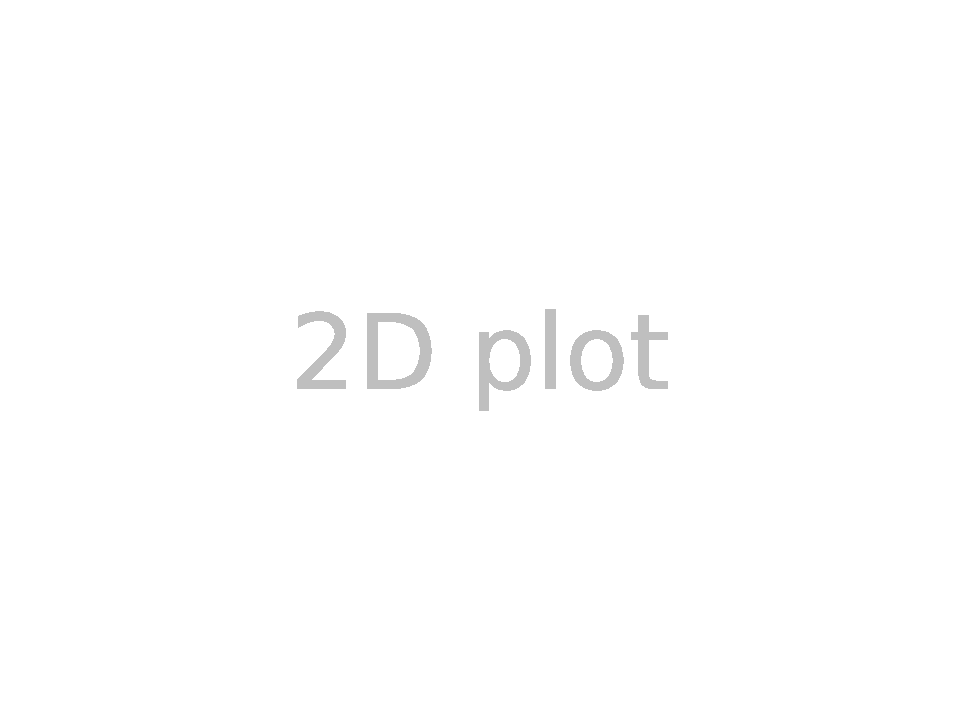
\includegraphics[width=\textwidth]{Plotter2D}
	\caption{\textbf{TREPR-Signal von {@METADATA['SAMPLE']['Name']} bei {@METADATA['TEMPERATURE']['Temperature']}.} 900 spp; MW: {@METADATA['BRIDGE']['Attenuation']}, {@METADATA['BRIDGE']['Power']}; VAmp: {@METADATA['VIDEO AMPLIFIER']['Amplification']}, {@METADATA['VIDEO AMPLIFIER']['Bandwidth']}; Laser: {@METADATA['PUMP']['Wavelength']} (OPO Pos. {@METADATA['PUMP']['Tunable position']}), {@METADATA['PUMP']['Repetition rate']}, {@METADATA['PUMP']['Power']} pro Puls.} 
\end{figure}

\clearpage
\section*{Experimentelle Parameter}

\begin{minipage}{\textwidth}
\begin{tabbing}
\hspace{3.5cm} \= \kill
\textbf{Sample}\\
%{for key, value in METADATA['SAMPLE'].items()}%
	{@key} \> {@value}\\
%{endfor}%
\end{tabbing}
\end{minipage}
	
\begin{multicols}{2}

%{for KEY, VALUE in METADATA['PARAMETER'].items() recursive}%
	\begin{minipage}{.49\textwidth}
	\textbf{{@KEY}}\\
	%{for key2, value2 in VALUE.items()}%
		{@key2}: {@value2}\\
	%{endfor}%
	\end{minipage}
%{endfor}%
\end{multicols}

\begin{minipage}{\textwidth}
\textbf{Comment}\\
%{for line in METADATA['COMMENT']}%
	{@line}\\
%{endfor}%
\end{minipage}





\begin{figure}[H]
	
\includegraphics[width=\textwidth]{Plotter1D}
	\caption{\textbf{TREPR-Signal von {@METADATA['SAMPLE']['Name']} bei {@METADATA['TEMPERATURE']['Temperature']}: Schnitt bei {@PROCESSINGPARAMETERS['Schnitt bei']} (gemittelt über {@PROCESSINGPARAMETERS['gemittelt über']}).} 900 spp; MW: {@METADATA['BRIDGE']['Attenuation']}, {@METADATA['BRIDGE']['Power']}; VAmp: {@METADATA['VIDEO AMPLIFIER']['Amplification']}, {@METADATA['VIDEO AMPLIFIER']['Bandwidth']}; Laser: {@METADATA['PUMP']['Wavelength']} (OPO Pos. {@METADATA['PUMP']['Tunable position']}), {@METADATA['PUMP']['Repetition rate']}, {@METADATA['PUMP']['Power']} pro Puls.} 
\end{figure}

\section*{Prozessierung}

%{for item in PROCESSINGSTEPS}%
	{@item}\\
%{endfor}%


\end{document}